\chapter{引言}

在我们周围有各种各样的物体。例如,课本、书桌、黑板、人们生活的地球、空中的太阳、月亮,等等。
这些物体都有一定的形状和大小,并且在不同的位置上,如黑板是长方形的、地球的半径约 6370 公里、课本在书桌上等。
这些物体还有其他的性质,如书桌是木制的、地球上有生命、太阳能发光、月亮不能发光等。

在生产建设和日常生活中,我们常常需要研究物体的形状、大小和位置关系。
例如,修建房屋、建筑堤坝、制造机器零件时,都要考虑它们的形状、大小和确定它们的施工或安装位置。
在“几何” \footnotemark 里,只研究物体的形状、大小和位置关系,而不考虑物体的其他性质。
\footnotetext{“几何” 是一个翻译名词。它是我国明代科学家 徐光启(公元 1562 ~ 1633 年)首先用的,原意是 “测量土地的技术”。}

对于一个物体,当只研究它的形状、大小而不考虑其他性质时,我们就说它是\zhongdian{几何体},几何体简称为\zhongdian{体}。
图 \ref{fig:czjh1-intro-1} 中的木块、圆钢、篮球,当只考虑它们的形状、大小时,我们就分别说它们是长方体、圆柱体和球体。

\begingroup
\renewcommand{\thefigure}{\arabic{figure}\;}

\begin{figure}[htbp]
    \centering
    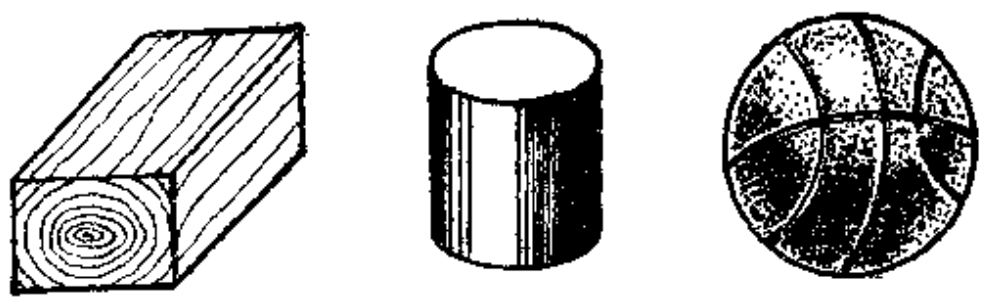
\includegraphics[width=0.5\textwidth]{../pic/czjh1-intro-1}
    \caption{}\label{fig:czjh1-intro-1}
\end{figure}

体是由\zhongdian{面}围成的,面有平的、有曲的。
例如长方体是\zhongdian{由六个平的面}围成的,圆柱体是由两个平的面和一个曲的面围成的(图 \ref{fig:czjh1-intro-2})。

\begin{figure}[htbp]
    \centering
    \begin{tikzpicture}
	\begin{scope}
		\pgfmathsetmacro{\a}{2}
		\pgfmathsetmacro{\b}{1}
		\pgfmathsetmacro{\c}{1}
		\draw [dashed] (0,0,0) -- (0,0,-\c) -- (0,\b,-\c);
		\draw [dashed] (0,0,-\c) -- (\a,0,-\c);
		\draw (0,0,0) -- (\a,0,0) -- (\a,\b,0) -- (0,\b,0) -- cycle;
		\draw (\a,0,0) -- (\a,\b,0) -- (\a,\b,-\c) -- (\a,0,-\c) --cycle;
		\draw (0,\b,0) -- (0,\b,-\c) -- (\a,\b,-\c) -- (\a,\b,0) -- cycle;
	\end{scope}

	\tdplotsetmaincoords{60}{0}
	\begin{scope}[tdplot_main_coords, scale=0.7, xshift=6cm]
		\pgfmathsetmacro{\r}{1}
		\pgfmathsetmacro{\h}{2}

		\draw plot[smooth,variable=\t,domain=\tdplotmainphi:\tdplotmainphi-180]
				({\r*cos(\t)},{\r*sin(\t)},\h)
			-- plot[smooth,variable=\t,domain=\tdplotmainphi-180:\tdplotmainphi]
				({\r*cos(\t)},{\r*sin(\t)},0) -- cycle;
		\draw plot[smooth,variable=\t,domain=0:360] ({\r*cos(\t)},{\r*sin(\t)},\h);
		\draw [dashed] plot[smooth,variable=\t,domain=0:360] ({\r*cos(\t)},{\r*sin(\t)},0);
	\end{scope}
\end{tikzpicture}


    \caption{}\label{fig:czjh1-intro-2}
\end{figure}

\endgroup

面和面相交于\zhongdian{线}。 线有直的、有曲的。
例如,长方体相邻的两个面相交于一条直的线(长方体的棱)。
圆柱体的侧面和一个底面相交于一条曲的线(图 \ref{fig:czjh1-intro-2})。

线和线相交于\zhongdian{点}。
如长方体相邻的两条棱相交于一个点(长方体的顶点)。

点、线、面或若干个点、线、面组合在一起,就成为\zhongdian{几何图形}。

在我们将要学习的几何里,只研究在同一个平面内的图形——\zhongdian{平面图形}。
在小学里学过的三角形、长方形和圆都是平面图形,而长方体、圆柱和球都不是平面图形。
下面,我们将要学习许多常用的平面图形及其性质。


